\chapter{内存寻址}

\section{内存地址}

    在使用80x86微处理器时,我们必须区分以下三种不同的地址:

\begin{itemize}
    \item 逻辑地址(logical address)
    \subitem 包含在机器语言指令中用来指定一个操作数或一条指令的地址。\emph{每一个逻辑地址都由一个段(segment)和偏移量(offset或displacement)组成,偏移量指明了从段开始的地方到实际地址之间的距离。}
    \item 线性地址(linear address)(也称虚拟地址 virtual address)
    \subitem 是一个32位无符号整数,可以用来表示高达4GB的地址。
    \item 物理地址(physical address)
    \subitem 用于内存芯片级内存单元寻址。从微处理器的地址引脚发送到内存总线上的电信号相对应。
\end{itemize}

    \emph{内存控制单元(MMU)通过分段单元(segmentation unit)的硬件电路把一个逻辑地址转换成线性地址,然后分页单元(paging unit)的硬件电路把线性地址转化为物理地址}。

    在多处理器中,所有CPU都共享同一内存:这意味着RAM可以由独立的CPU并发访问。但因为RAM上的读写必须串行执行,因此需要内存仲裁器(memory arbiter)的硬件电路插在总线和RAM芯片之间。

    内存仲裁器的作用是:\emph{如果某个RAM空闲,就准予CPU访问。若RAM忙于另一个CPU提出的请求服务,就延迟这个CPU的访问}

\section{硬件中的分段}

    从80286模型开始,Intel处理器以实模式\footnote[1]{\emph{实模式(Real Mode)是x86体系结构中的一种工作模式,它是早期x86处理器的默认工作模式。在实模式下,处理器以16位的方式进行操作,可以直接访问1MB的物理内存。在实模式下,内存寻址是通过段地址和偏移地址的组合来实现的。段地址由段寄存器(如CS、DS、ES等)保存,偏移地址由指令中的操作数给出。通过将段地址左移4位后与偏移地址相加,可以计算出实际的物理地址}}(real mode)和保护模式(protected mode)执行地址转换。

\subsection{段选择符和段寄存器}

    一个逻辑地址由\emph{一个段标识符(16位长的字段,段选择符(Segment Selector))和一个指定段内相对地址的偏移量(32位长的字段)组成。}

\begin{figure}[!htbp]
    \centering
    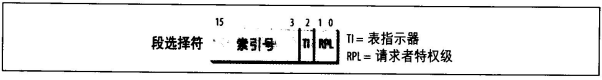
\includegraphics[width=0.8\textwidth]{image/chapter02/段选择符格式.png}
    \caption{段选择符格式}
\end{figure}

    为了方便段选择符,段寄存器用于存放段选择符。其拥有六个寄存器:

\begin{table*}[!htbp]
    \begin{center}
        \begin{tabular}{c | c}
            cs & 代码段寄存器,指向包含程序指令的段 \\
            ss & 栈段寄存器,指向包含当前程序栈的段 \\
            ds & 数据段寄存器,指向包含静态数据或者全局数据段 \\
            es, fs, gs & 一般用途,可以指向任意数据段 
        \end{tabular}
    \end{center}
\end{table*}

    cs寄存器:\emph{包含一个两位的字段,用以指明CPU的当前特权级\footnote[1]{\emph{值为0表示最高优先级,值为3为最低。Linux只用0和3表示内核态和用户态。}}(Current Privilege Level, CPL)。}

\subsection{段描述符}

    每个段由一个8字节的段描述符(Segment Descriptor)表示,描述了段的特征。

    段描述符放在全局描述符表(Global Descriptor Table,GDT)或局部描述符表(Local Descriptor Table,LDT)中。

    通常只定义一个GDT,每个进程除了存放在GDT中的段之外如果还需附加,就可以使用LDT。GDT在主存中的地址和大小存放在gdtr控制寄存器中,LDT地址和大小存放在ldtr控制寄存器中。

\begin{table*}[!htbp]
    \begin{center}
        \caption{段描述符字段}
        \begin{tabular}{c l}
            \hline
            \emph{字段名} & \emph{描述} \\
            Base & 包含段的首字节的线性地址 \\ 
            G & 粒度标志;若清零,则段大小以字节为单位,否则以4096字节倍数计 \\
            Limit & 存放段中最后一个内存单元的偏移量,从而决定段的长度。\\
            S & 系统标志;置零表示系统段,否则是普通代码段或数据段 \\
            Type & 描述了段的类型特征和存取权限 \\
            DPL & 描述符特权级(Dsecriptor Privilege Level)字段;用于限制这个段的存取。\\
            & 其表示为访问这个段要求的CPU最小优先级。若DPL设为0的段只能\\
            & 当CPL为0时(即内核态)可访问 \\
            P & Segment-Present标志;等于0表示段当前不在主存中\\ 
            & \emph{Linux总是把这个标志设置为1,因为其从不把整个段交换到磁盘}\\
            D或B & 取决于是代码段还是数据段。D或B的含义在两种情况下略有区别\\
            & 如果偏移量32位则置1,否则清零 \\
            \hline
        \end{tabular}
    \end{center}
\end{table*}

    有几种不同类型的段以及对应的段描述符:

\begin{itemize}
    \item 代码段描述符
    \subitem 表示这个段描述符表示代码段,S标志置1
    \item 数据段描述符
    \subitem 表示这个段描述符表示数据段,S标志置1
    \item 任务状态段描述符(TSSD)
    \subitem 表示这个段描述符表示任务状态段(Task State Segment, TSS),也就是该段用于保存处理器寄存器的内容。\emph{只能出现在GDT中,根据相应进程是否在CPU上,其Type字段值为11或9,S标志置零}
    \item 局部描述符表描述符(LDTD)
    \subitem 表示这个段描述符包含一个LDT段,其只出现在GDT中。相应的Type字段值为2,S标志置0
\end{itemize}

\begin{figure}[!htbp]
    \centering
    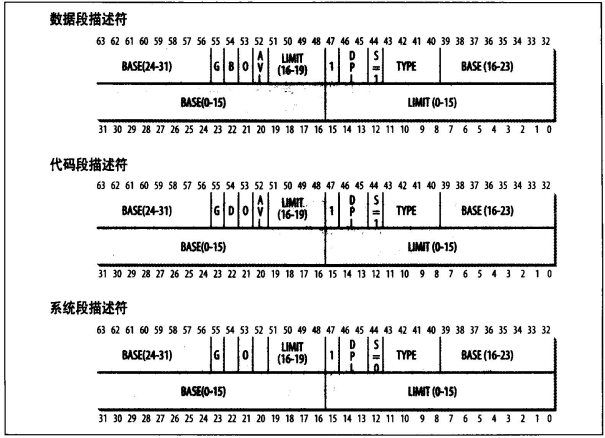
\includegraphics[width=0.8\textwidth]{image/chapter02/段描述符格式.png}
    \caption{段描述符格式}
\end{figure}

\subsection{快速访问段描述符}

    \emph{逻辑地址由16位段选择符和32位偏移量组成,段寄存器仅仅存放段选择符。}

    为了加速逻辑地址$\rightarrow$线性地址,80x86处理器提供了附加的非编程的寄存器,供6个可编程的段寄存器使用。每一个非编程的寄存器含有八个字节的段描述符,由对应的段寄存器中的段选择描述符来指定。

    每当一个段选择符被装入段寄存器,相应的段描述符就由内存装入对应的非编程CPU寄存器。这时,针对该段的逻辑地址转换就可以仅访问该非编程寄存器即可(除非段寄存器内容发生更改)。

\begin{figure}[!htbp]
    \centering
    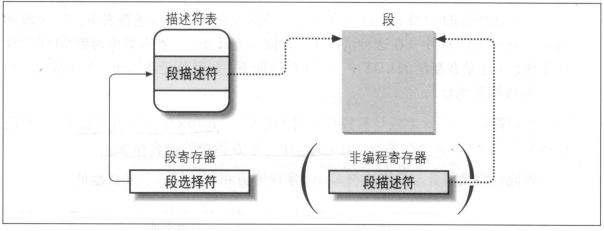
\includegraphics[width=0.8\textwidth]{image/chapter02/段选择符和段描述符.png}
    \caption{段选择符和段描述符}
\end{figure}

\begin{table*}[!htbp]
    \begin{center}
        \caption{段选择符字段}
        \begin{tabular}{c l}
            \hline
            \emph{字段名} & \emph{描述} \\
            index & 指定了描述放在GDT/LDT中对应的段描述符入口 \\
            TI & TI((Table Indicator)标志,指明段描述符是在GDT(TI = 0)中或LDT(TI = 1)中) \\
            RPL & 请求者特权级,当相应的段选择符装入到cs寄存器中时指示出CPU当前的特权级 \\
            & 还可以用于访问数据段时选择地削弱特权级 \\
            \hline
        \end{tabular}
    \end{center}
\end{table*}

    由于段描述符是8字节长,因此在GDT/LDT中的相对地址由段选择符的最高13位数值乘以8得到

    \emph{GDT的第一项总是设置为0,这就确保了空段选择符的逻辑地址会被认为是无效的。因此引起一个处理器异常。}

\subsection{分段单元}

    分段单元(segmentation unit)执行以下步骤:

\begin{itemize}
    \item 首先检查TI字段以决定段描述符保存在哪个描述符表。
    \item 从段选择符的index字段计算段描述符的地址
    \item 把逻辑地址的偏移量与段描述符Base字段的值相加就得到了线性地址
\end{itemize}

\begin{figure}[!htbp]
    \centering
    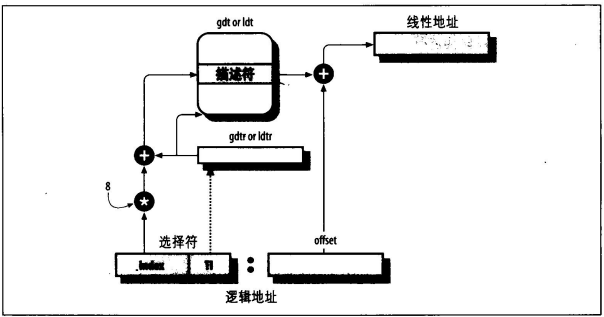
\includegraphics[width=0.8\textwidth]{image/chapter02/逻辑地址的转换.png}
    \caption{逻辑地址的转换}
\end{figure}

    注意:\emph{如果有了不可编程寄存器,只有当段寄存器内容被改变时才需执行前两个操作。}

\section{Linux中的分段}

    实际上分段和分页在某种程度上有点多余,因为都可以划分进程的物理地址空间:\emph{分段可以给每个进程分配不同的线性地址空间, 而分页可以把同一线性地址空间映射到不同的物理空间。}Linux更喜欢分页:

\begin{itemize}
    \item 当所有进程使用相同段寄存器值,内存管理变得更简单,也就是其能共享同样的一组线性地址
    \item RISC架构对分段的支持有限\footnote[1]{\emph{2.6version的Linux只有80x86架构才需要使用分段}}
\end{itemize}

    运行到用户态的所有Linux进程都使用一对相同的段来对指令和数据寻址。也就是用户代码段和用户数据段。相对地,也有内核代码段和内核数据段。

\begin{table*}[!htbp]
    \begin{center}
        \caption{四个主要的Linux段的描述符字段的值}
        \begin{tabular}{c c c c c c c c c}
            \hline
            \emph{段} & \emph{Base} & \emph{G} & \emph{Limit} & \emph{S} & \emph{Type} & \emph{DPL} & \emph{D/B} & \emph{P} \\
            用户代码段 & 0x00000000 & 1 & 0xfffff & 1 & 10 & 3 & 1 & 1 \\
            用户数据段 & 0x00000000 & 1 & 0xfffff & 1 & 2 & 3 & 1 & 1 \\
            内核代码段 & 0x00000000 & 1 & 0xfffff & 1 & 10 & 0 & 1 & 1 \\
            内核数据段 & 0x00000000 & 1 & 0xfffff & 1 & 2 & 0 & 1 & 1 \\
            \hline
        \end{tabular}
    \end{center}
\end{table*}

    相应的段选择符由宏\_\_USER\_CS,\_\_USER\_DS,\_\_KERNEL\_CS和\_\_KERNEL\_DS分别定义。

    \emph{所有的段都从0x00000000开始,也就是说,Linux下逻辑地址与线性地址是一致的,即逻辑地址的偏移量字段与对应的线性地址的值总是一致的。}

    对指令或数据结构的指针进行保存时,内核不需要设置逻辑地址的段选择符,因为CS寄存器含有当前的段选择符。因为已经隐含在CS寄存器中。"在内核态执行"的段只有一种,叫做代码段,由\_\_KERNEL\_CS定义,因此当切换为内核态时,只需要将该宏装入CS即可。

    同样的,对于指向内核数据结构的指针,隐式使用DS,有宏\_\_KERNEL\_DS。

\subsection{Linux GDT}

    多处理器中,每个CPU对应一个GDT。所有的GDT都存放在\emph{`cpu\_gdt\_table`}数组中,而所有的GDT地址和大小(初始化gdtr寄存器时使用)被存放在\emph{`cpu\_gdt\_descr`}数组中。

\begin{lstlisting}[language=C++]
// for i386 GDT_ENTRIES
#define GDT_ENTRIES 32 

// for x86_64 GDT_ENTRIES
#define GDT_ENTRIES 16

// 8 byte segment descriptor
struct desc_struct { 
	u16 limit0;
	u16 base0;
	unsigned base1 : 8, type : 4, s : 1, dpl : 2, p : 1;
	unsigned limit : 4, avl  : 1, l : 1, d   : 1, g : 1, base2 : 8;
} __attribute__((packed)); 

extern struct desc_struct cpu_gdt_table[NR_CPUS][GDT_ENTRIES];

struct Xgt_desc_struct {
	unsigned short size;
	unsigned long address __attribute__((packed));
	unsigned short pad;
} __attribute__ ((packed));

extern struct Xgt_desc_struct idt_descr, cpu_gdt_descr[NR_CPUS];
\end{lstlisting}

    如下是GDT的布局示意图,每个GDT都包含18个描述符和14个空的,未使用的,或保留的。\emph{插入未使用的项目的是为了使经常一起访问呢的描述符能够处于同一个32字节的硬件高速缓存行中}

\begin{figure}[!htbp]
    \centering
    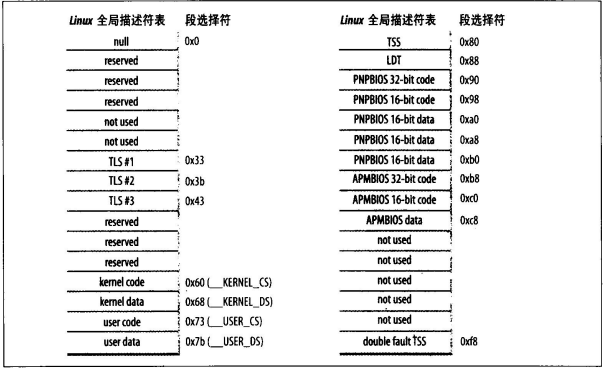
\includegraphics[width=0.8\textwidth]{image/chapter02/全局描述符表.png}
    \caption{全局描述符表}
\end{figure}

    每一个GDT中包含的18个段描述符指向下列的段:

\begin{itemize}
    \item 用户态和内核态下的代码段和数据段共四个
    \item 任务状态段(TSS),每个处理器一个。
    \subitem TSS相应的线性地址空间都是内核数据段相应线性空间的一个小子集。所有的状态任务段都顺序地放在init\_tss数组中。注意:\emph{第n个CPU的TSS描述符的Base字段指向init\_tss数组的第n个元素,G标志清零,Limit字段置为0xeb,Type字段置为9或11且DPL置0}
    \item 1个包括缺省局部描述符的段,通常被所有进程共享的段
    \item 3个局部线程存储(Thread-Local Storage, TLS)段
    \subitem 该机制允许多线程应用程序使用最多3个局部线程的数据段。系统调用set\_thread\_area()和get\_thread\_area()分别创建和撤销一个TLS段
    \item 与高级电源管理(AMP)相关的三个段
    \subitem 由于BIOS代码使用段,所以Linux APM驱动程序调用BIOS函数来获取或设置APM时,可以自定义的代码段和数据段
    \item 与支持即插即用(PnP)功能的BIOS服务程序相关的五个段
    \subitem 当PnP设备驱动程序调用BIOS函数来检查PnP设备使用的资源时,就可以使用自定义的代码段和数据段
    \item 被内核用来处理"双重错误"异常\footnote[1]{\emph{处理异常的程序引发了另一个异常,产生的双重错误}}的特殊TSS段
\end{itemize}

\subsection{Linux LDT}

    大多数用户态Linux不使用局部描述符表,内核定义了一个缺省的LDT供进程共享。缺省的局部描述符放在\emph{`default\_ldt'}数组中,其包含五个项,但内核仅仅有效地使用了其中两个项。

\begin{itemize}
    \item 用于iBCS执行文件的调用门
    \item Solaris/x86可执行文件的调用门
\end{itemize}

    调用门时80x86微处理器提供的一种机制,可以在调用与预定义函数时改变CPU的特权级。

\begin{lstlisting}[language=C++]
// 8 byte segment descriptor
struct desc_struct { 
	u16 limit0;
	u16 base0;
	unsigned base1 : 8, type : 4, s : 1, dpl : 2, p : 1;
	unsigned limit : 4, avl  : 1, l : 1, d   : 1, g : 1, base2 : 8;
} __attribute__((packed)); 

extern struct desc_struct default_ldt[];
\end{lstlisting}

    但是,如同Wine这样的程序,需要创建局部描述符。modify\_ldt()系统调用允许进程创建自己的局部描述符。

    任何被modify\_ldt()创建的自定义局部描述符仍然需要自己的段。

\begin{lstlisting}[language=C++]
/*
* ldt.h
*
* Definitions of structures used with the modify_ldt system call.
*/
#ifndef _LINUX_LDT_H
#define _LINUX_LDT_H

/* Maximum number of LDT entries supported. */
#define LDT_ENTRIES	8192
/* The size of each LDT entry. */
#define LDT_ENTRY_SIZE	8

#ifndef __ASSEMBLY__
struct user_desc {
    unsigned int  entry_number;
    unsigned long base_addr;
    unsigned int  limit;
    unsigned int  seg_32bit:1;
    unsigned int  contents:2;
    unsigned int  read_exec_only:1;
    unsigned int  limit_in_pages:1;
    unsigned int  seg_not_present:1;
    unsigned int  useable:1;
};

#define MODIFY_LDT_CONTENTS_DATA	0
#define MODIFY_LDT_CONTENTS_STACK	1
#define MODIFY_LDT_CONTENTS_CODE	2

#endif /* !__ASSEMBLY__ */
#endif  
\end{lstlisting}

\section{硬件中的分页}

    分页单元(paging unit)把线性地址转换为物理地址。其中的一个关键任务是把所请求的访问类型与线性地址的访问权限比较,若内存访问无效,则产生缺页异常。

    \emph{线性地址被分成以固定长度为单位的组,称为页(page)。}页内部连续的线性地址被映射到连续的物理地址中。内核就能够指定一个页的物理地址和存取权限,而不用指定页所包含的全部线性地址的存取权限。

    一般地,使用属于"页"既指一组线性地址,又指包含在这组地址中的数据。

    分页单元把所有的RAM分成固定长度的页框(page frame)。每个页框包含一个页,也就是说,一个页框的长度和页的长度是一致的。

    把线性地址映射到物理地址的数据结构称为页表(page table)。

    从80386开始,所有的80x86处理器都支持分页,通过设置cr0寄存器的PG标志启用。当PG=0时,线性地址被解释为物理地址

\subsection{常规分页}

    32位的线性地址被分成3个域:

\begin{itemize}
    \item Directory(目录)
    \subitem 最高10位
    \item Table(页表)
    \subitem 中间十位
    \item Offset(偏移量)
    \subitem 最低12位
\end{itemize}

    线性地址的转换分两步,每一步都基于一种转换表。第一种转换表称为页目录表(page directory),第二种转换表称为页表(page table)

    \emph{使用这种二级模式的目的在于减少每个进程页表所需RAM的数量}。

    正在使用的页目录的物理地址存放在控制寄存器cr3中。

\begin{figure}[!htbp]
    \centering
    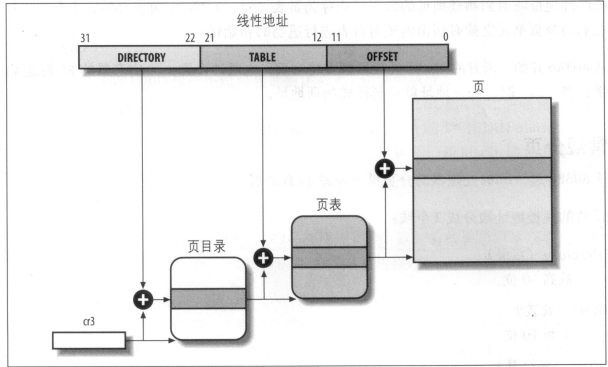
\includegraphics[width=0.8\textwidth]{image/chapter02/80x86处理器分页.png}
    \caption{80x86处理器分页}
\end{figure}

    线性地址内的Directory字段决定页目录中的目录项,而目录项指向适当的页表。地址的Table字段依次又决定页表中的表项,表项含有页所在页框的物理地址。Offset字段决定页框内的相对位置。

    Directory字段和Table字段都是10位长,因此页目录和页表都可以多达1024项。

    页目录项和页表有同样的结构,每项都包含下面的字段:

\begin{itemize}
    \item Present标志
    \subitem 若被置1,所在页就在主存中;若地址转换所需的页表项或页目录项中Present标志清零,则分页单元就把该线性地址放在控制寄存器cr2中,产生14号缺页异常
    \item 包含页框物理地址最高20位的字段
    \subitem 一个页框4KN大小,因此物理地址是4096的倍数(低12位总是0).
    \item Accessed标志
    \subitem 每当分页单元对相应页框进行寻址时设置。必须被操作系统设置。
    \item Dirty标志
    \subitem 只用于页表项。每当一个页框进行写操作时设置。必须被操作系统设置。
    \item Read/Write标志
    \subitem 含有页或页表的存取权限
    \item User/Supervisor标志
    \subitem 含有访问页或页表所需的特权级
    \item PCD和PWT标志
    \subitem 控制硬件高速缓存处理页或页表的方式
    \item Page Size标志
    \subitem 只用于页目录项。
    \item Global标志
    \subitem 只用于页表项。用来防止页从TLB高速缓存中刷新出去。只有cr4寄存器在页全局启用(Page Global Enable, PGE)标志置位时才有效
\end{itemize}